% !TeX root = Applied Graph Theory.tex

\title{\textbf{Applied Graph Theory}}

\date{}
\maketitle

\begingroup
\let\clearpage\relax
\tableofcontents
\endgroup

\clearpage

\renewcommand{\nomname}{List of Symbols}
\nomenclature[01]{$V(G)$}{Vertex set of graph $G$}
\nomenclature[02]{$E(G)$}{Edge set of graph $G$}
\nomenclature[03]{$\sim$}{is adjacenct to}
\nomenclature[04]{$\deg(v)$}{Degree of vertex $v$}
\nomenclature[05]{$\ecc(v)$}{Eccentricity of vertex $v$}
\nomenclature[06]{$\rad(G)$}{Radius of graph $G$}
\nomenclature[07]{$\diam(G)$}{Diameter of graph $G$}
\nomenclature[08]{$A(G)$}{Adjacency matrix graph $G$}

\nomenclature[10]{$G - v$}{Graph obtained from $G$ by deleting vertex $v$ and all edges incident with $v$}
\nomenclature[11]{$G - e$}{Graph obtained from $G$ by deleting edge $e$}

\nomenclature[20]{$K_n$}{Complete graph of order $n$ (size $\binom{n}{2}$)}
\nomenclature[21]{$P_n$}{Path graph of order $n$ (size $n - 1$)}
\nomenclature[22]{$C_n$}{Cycle graph of order $n$ (size $n$)}
\printnomenclature[10em]

\clearpage

\section{Introdcution}\label{sec:Intro}
A \emph{graph} is an ordered pair $G = (V, E)$ where $V$ is a nonempty set called the \emph{vertex set}, whose elements are the \emph{vertices} of $G$, and $E$ is a set of unordered pairs of distinct vertices of $G$, whose elements are the \emph{edges} of $G$. The \emph{order} of $G$ is its number of vertices and the \emph{size} of $G$ is its number of edges.

Two vertices $u$ and $v$ of $G$ are \emph{adjacent}, denoted by $u \sim v$, if $(u,v) \in E(G)$ -- we may also denote the edge $(u,v)$ as simply $uv$. Note that $uv = vu$. If there is no edge between $u$ and $v$, then they are \emph{nonadjacent}, denoted by $u \nsim v$. The vertex $v$ and the edge $uv$ are said to be \emph{incident} with each other. The \emph{degree} of a vertex $v$ is the number of edges incident with it, or equivalently, the number of vertices adjacent with it, and is denoted by $\deg(v)$.

\begin{Lemma}[Handshaking Lemma]
The sum of the degrees of all vertices of a graph is twice its size.
\end{Lemma}

\begin{proof}
Exercise.
\end{proof}

\section{Cartesian Products}\label{sec:CartProds}

The \emph{Cartesian product} of two graphs $G$ and $H$ is the graph denoted by $G \times H$, whose vertex set is $V(G) \times V(H)$ (the Cartesian product of the vertex sets $V(G)$ and $V(H)$, consisting of all ordered pairs $(u, v)$ where $u$ is a vertex of $G$ and $v$ is a vertex of $H$), in which two vertices $(u_1, v_1)$ and $(u_2, v_2)$ are adjacent if and only if either $u_1 = u_2$ and $v_1 \sim v_2$ or $u_1 \sim u_2$ and $v_1 = v_2$.

\begin{Exercise}
Prove that if $G$ is a graph of order $p_1$ and size $q_1$, and $H$ is a graph of order $p_2$ and size $q_2$, then $G \times H$ is a graph of order $p_1 p_2$ and size $p_1 q_2 + p_2 q_1$.
\end{Exercise}

\section{Trees}\label{sec:Trees}

A \emph{tree} is a connected, acyclic graph. There are several well known characterisations or alternative definitions of trees. We take the given definition as the basic one and prove its equivalence to some others.

\begin{Theorem}\label{thm:UniPath}
A graph $T$ is a tree if and only if there is a unique path joining every two vertices of $T$.
\end{Theorem}
\begin{proof}
First, suppose that $T$ is a tree, and let $u$ and $v$ be vertices of $T$. Since $T$ is connected, there is a path, say $P_1$, joining $u$ and $v$. Now we must show that this path is unique. Assume to the contrary that there exists another path $P_2$ from $u$ to $v$. When traversing $P_1$ from $u$ to $v$, let $w$ be the first vertex that is present on $P_1$ but not $P_2$. Let $x$ be the vertex on $P_1$ preceding $w$, and note that $x$ is on $P_2$ as well. Let $y$ be the next vertex common to both $P_1$ and $P_2$ when traversing $P_1$ from $x$ to $v$. Then the portion of $P_1$ from $x$ to $y$ together with the portion of $P_2$ from $y$ to $x$ forms a cycle in the tree $T$, which is a contradiction. Thus, $P_1$ is the unique path joining $u$ and $v$.

Conversely, suppose that $T$ is a graph in which there is a unique path joining any two vertices. Clearly, $T$ is connected. To show that $T$ is acyclic, suppose that $v_1, v_2, \ldots, v_n$ is a cycle in $T$. Then we get two different paths joining $v_1$ and $v_n$, namely the path $v_1, v_2, \ldots, v_n$ and the path $v_1, v_n$ (since $v_1 \sim v_n$ in the cycle). This contradicts our assumption. Thus, $T$ must be acyclic and hence is a tree.
\end{proof}

The next two results show that the size of a tree is always one less than its order, and that conversely, this property together with either connectedness or acyclicity implies that the graph is a tree.
\begin{Theorem}\label{thm:Conn;p=q+1}
A $(p, q)$-graph $T$ is a tree if and only if it is connected and $p = q + 1$.
\end{Theorem}
\begin{proof}
Let $T$ be a tree with $p$ vertices and $q$ edges. Then $T$ is connected. We prove that $p = q + 1$ by induction. This is clearly true when $p = 1$. Assume it to be true for all trees of order less than $p$. Now in $T$, we know that every two vertices are joined by a unique path. Thus, if $e$ is any edge of $T$, then the graph $T - \{e\}$ obtained by deleting $e$ has exactly two components, say $T_1$ and $T_2$. Each one is a tree, since it is connected and acyclic. Let $T_i$ have $p_i$ vertices and $q_i$ edges, $i = 1, 2$. Then by the hypothesis, $p_i = q_i + 1$ (since $p_i < p$). But $p = p_1 + p_2$ and $q = q_1 + q_2 + 1$ (since the size of $T - \{e\}$ is one less than that of $T$). Thus, $p = q_1 + q_2 + 2 = q + 1$.

For the converse, suppose that $T$ is a connected $(p,q)$-graph with $p = q + 1$. We must show that is acyclic. Suppose to the contrary that $T$ has a cycle $C$ with $k$ vertices. Then $C$ has $k$ edges as well. Since $T$ is connected, there is a path from every vertex not on $C$ to some vertex of $C$. The shortest path from each vertex $v$ not on $C$ to a vertex on $C$ has a unique edge incident with $v$, which is not part of $C$. Since there are $p - k$ vertices in $T$ not on $C$, there are $p - k$ such edges. Thus $q \ge (p - k) + k = p$, which contradicts our assumption that $p = q + 1$. Thus, $T$ must be acyclic.
\end{proof}

In the following theorem, the proof of the direct part is identical to that of Theorem~\ref{thm:Conn;p=q+1}, except for the assertion being about acyclicity rather than connectedness. The proof of the converse part is entirely different.
\begin{Theorem}\label{thm:Acyc;p=q+1}
A $(p,q)$-graph $T$ is a tree if and only if it is acyclic and $p = q + 1$.
\end{Theorem}
\begin{proof}
Let $T$ be a tree with $p$ vertices and $q$ edges. Then $T$ is acyclic. We prove that $p = q + 1$ by induction. This is clearly true when $p = 1$. Assume it to be true for all trees of order less than $p$. Now in $T$, we know that every two vertices are joined by a unique path. Thus, if $e$ is any edge of $T$, then the graph $T - \{e\}$ obtained by deleting $e$ has exactly two components, say $T_1$ and $T_2$. Each one is a tree, since it is connected and acyclic. Let $T_i$ have $p_i$ vertices and $q_i$ edges, $i = 1, 2$. Then by the hypothesis, $p_i = q_i + 1$ (since $p_i < p$). But $p = p_1 + p_2$ and $q = q_1 + q_2 + 1$ (since the size of $T - \{e\}$ is one less than that of $T$). Thus, $p = q_1 + q_2 + 2 = q + 1$.

Conversely, suppose that $T$ is an acyclic $(p,q)$-graph with $p = q + 1$. To show that $T$ is connected, we need to prove that it is connected -- i.e., it has only one component. Let $T$ have $k$ components $T_1, \ldots, T_k$. Each one is acyclic, and being connected, is a tree. Thus from the first part of the theorem, we know that if $p_i$ and $q_i$ are respectively the order and size of the component $T_i$, $p_i = q_i + 1$. Now $p = p_1 + \cdots p_k = (q_1 + 1) + \cdots (q_k + 1) = q + k$. But we know that $p = q + 1$. Therefore, $k = 1$. Thus, $T$ is a tree.
\end{proof}

\begin{Exercise}
A \emph{pendant vertex} of a graph is a vertex of degree $1$. Prove that every non-trivial tree contains at least two pendant vertices.\\
{\tiny \textbf{Hint:} Observe that a non-trivial tree cannot have a vertex of degree zero. Use Handshaking Lemma and assume every degree is at least $2$ to get a contradiction.}
\end{Exercise}

\begin{Exercise}
The \emph{centre} of a graph $G$ is the set of all vertices of $G$ with minimum eccentricity -- i.e., the set of all vertices $v$ of $G$ with $\ecc v = \rad v$. Show that every tree has a centre consisting of either exactly one vertex or exactly two adjacent vertices.\\
{\tiny \textbf{Hint:} Observe that deleting all pendant vertices of a tree results in a new tree with the same centre.}
\end{Exercise}

\begin{Exercise}
If $G$ and $H$ are two trees of orders $n$ and $m$ respectively, what is the size of $G \times H$?
\end{Exercise}

\section{Blocks}\label{sec:Blocks}
A \emph{cutvertex} of a graph is a vertex whose removal increases the number of components, i.e., a vertex $v$ of $G$ such that $G - v$ has more components than $G$. If $G$ is connected, we can equivalently say that $v$ is a cutvertex if $G - v$ is disconnected. Similarly, a \emph{cutedge} or \emph{bridge} of a graph whose removal increases the number of components. A \emph{nonseparable} graph is a connected, non-trivial graph with no cutvertices. A maximal nonseparable subgraph of a graph is a \emph{block} of the graph. A nonseparable graph is itself said to be a block as well.

\begin{Example}\label{ex:Blocks}
The graph shown below has $6$ blocks and $3$ cutvertices ($v_1$, $v_2$, $v_3$).
\begin{center}
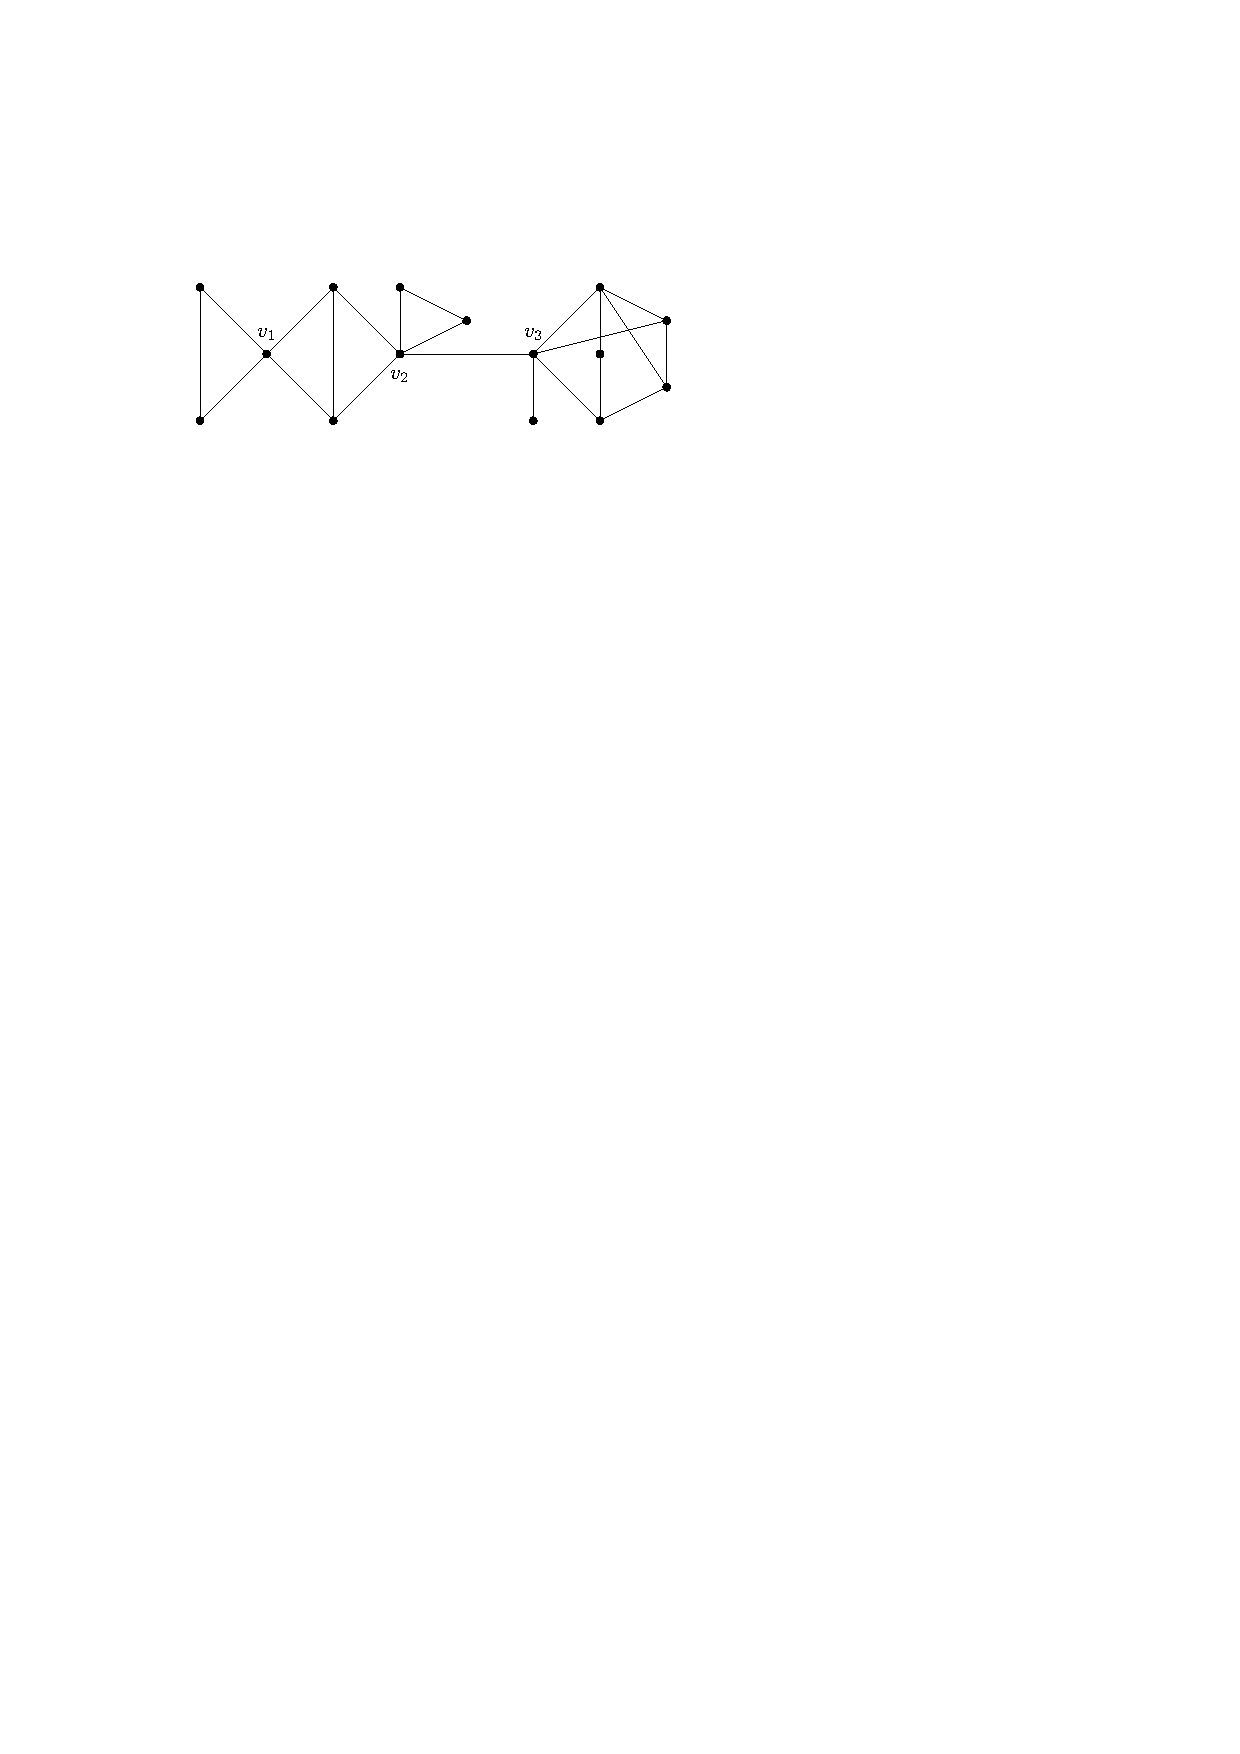
\includegraphics{6BlockGraph2.pdf}
\end{center}
The $6$ blocks of this graph are shown below.
\begin{center}
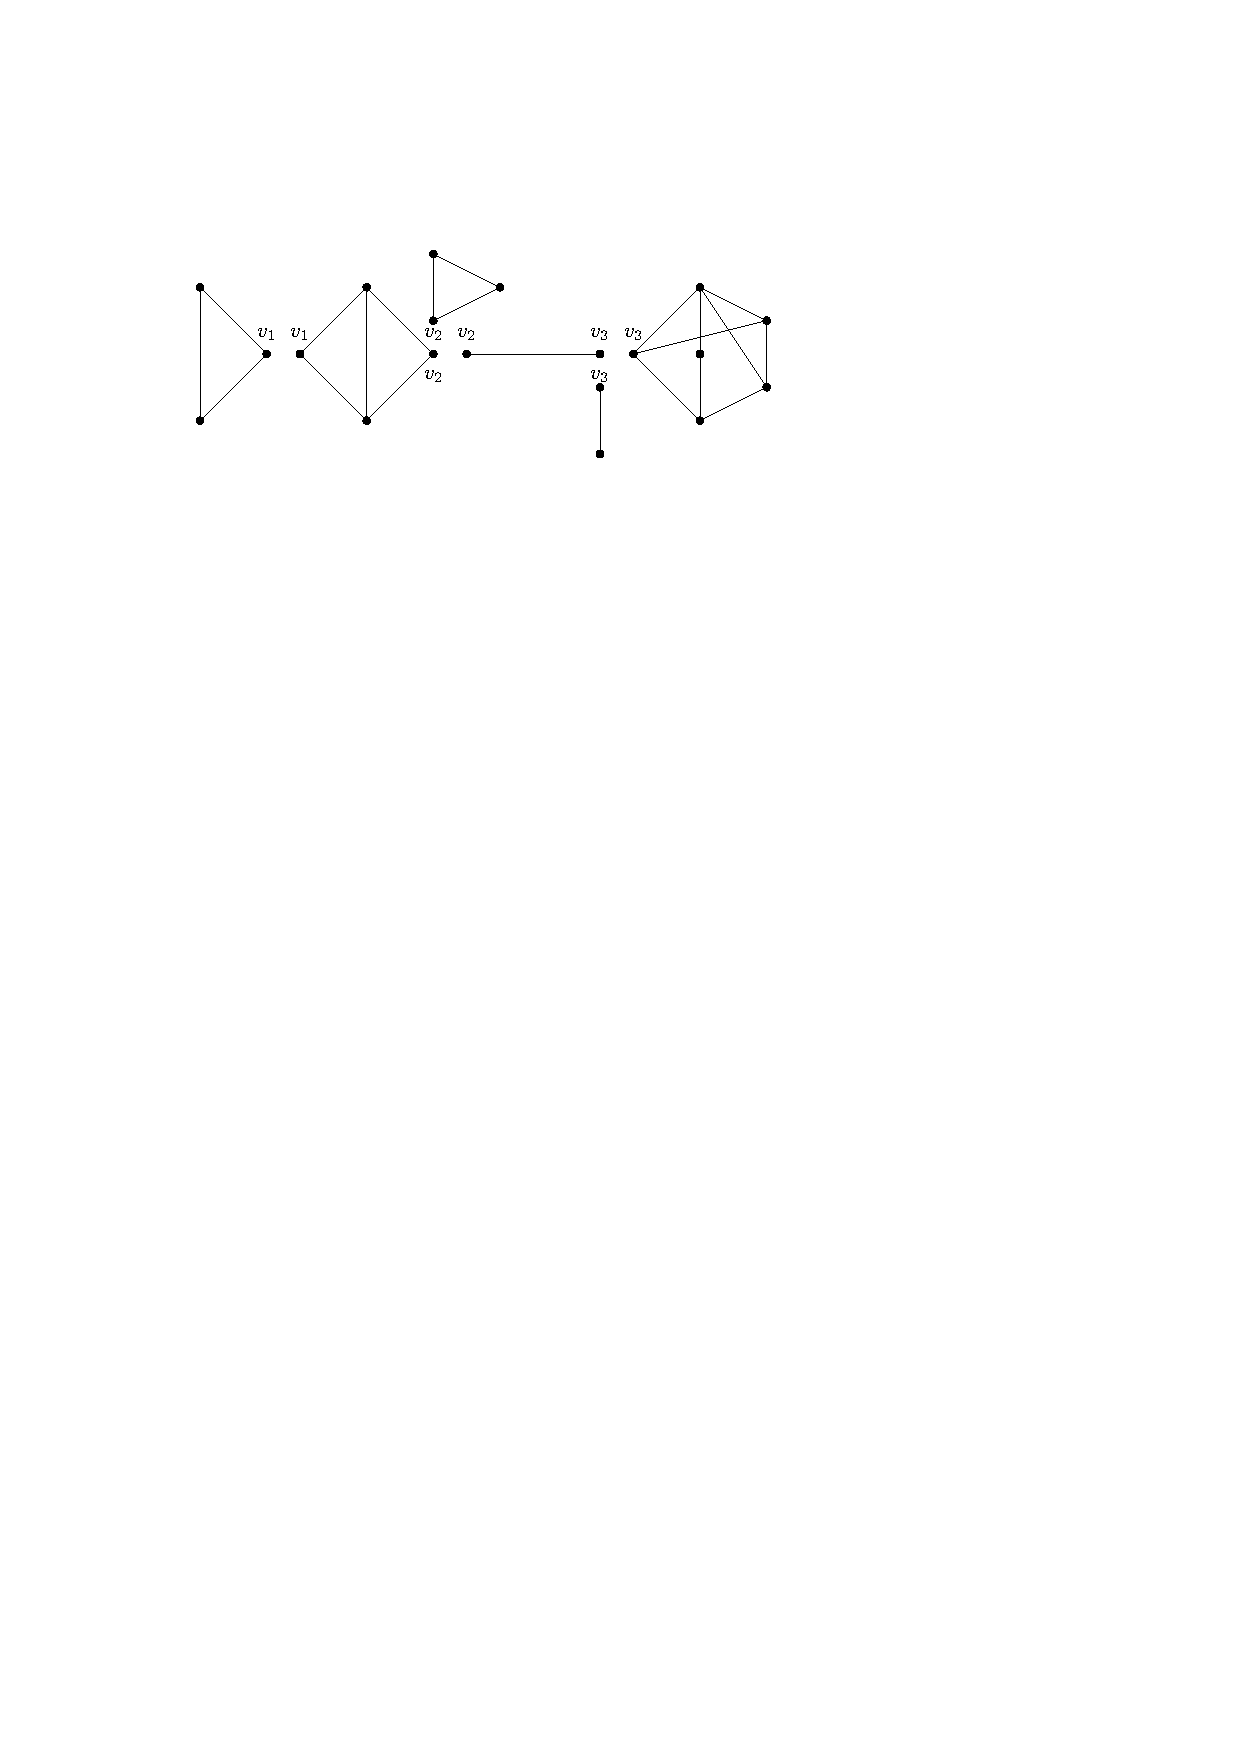
\includegraphics{6BlockGraph2-Blocks.pdf}
\end{center}
\end{Example}

\begin{Theorem}\label{thm:CutverChar}
If $G$ is a connected graph, and $v$ is any vertex of $G$, then the following are equivalent:
\begin{enumerate}[label=(\roman*)]
\item\label{it:CutverChar1} $v$ is a cutvertex of $G$.
\item\label{it:CutverChar2} There exist vertices $u$ and $w$ of $G$, distinct from $v$, such that every $u$-$w$ path passes through $v$.
\item\label{it:CutverChar3} There exists a partition of $V(G) - v$ into two non-empty subsets $U$ and $W$ such that for all $u \in U$ and $w \in W$, every $u$-$w$ path passes through $v$.
\end{enumerate}
\end{Theorem}

\begin{proof}
\cref{it:CutverChar1} $\implies $\cref{it:CutverChar3}. Since $v$ is a cutvertex, the graph $G - v$ is disconnected, i.e., it has two or more components. Let $U$ be all the vertices in any one of the components, and let $W$ be all the remaining vertices of $G - v$. Clearly, $\{U, W\}$ is a partition of $V(G) - v$. Now, if $u \in U$ and $w \in W$, then $u$ and $w$ are in different components of $G - v$, which implies that any path from $u$ to $w$ must pass through $v$.

\noindent \cref{it:CutverChar3} $\implies$ \cref{it:CutverChar2} is obvious as the latter is a special case of the former.

\noindent \cref{it:CutverChar2} $\implies$ \cref{it:CutverChar1}. Consider the graph $G - v$. As every $u$-$w$ path passes through $v$, none of them is present in $G - v$, and therefore $G - v$ is disconnected. Hence, $v$ is a cutvertex of $G$.
\end{proof}

\section{Adjacency Matrices}\label{sec:AdjMat}

The \emph{adjacency matrix} of a graph $G$ of order $n$, with vertex set $V = \{v_1, \ldots, v_n\}$, is the $n \times n$ matrix $A = A(G)$ whose $(i,j)$-entry is
\begin{equation*}
a_{ij} = \begin{cases}
1, & v_i \sim v_j \\
0, & v_i \nsim v_j.
\end{cases}
\end{equation*}

\begin{Example}\label{ex:GNM(6-11)AdjMat}
The adjacency matrix of the graph
\begin{center}
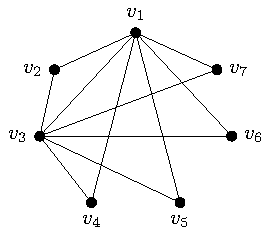
\includegraphics{GNM(6,11).pdf}
\end{center}
is
\begin{equation*}
A = \begin{bmatrix}
0 & 1 & 1 & 1 & 1 & 1 & 1 \\
1 & 0 & 1 & 0 & 0 & 0 & 0 \\
1 & 1 & 0 & 1 & 1 & 1 & 1 \\
1 & 0 & 1 & 0 & 0 & 0 & 0 \\
1 & 0 & 1 & 0 & 0 & 0 & 0 \\
1 & 0 & 1 & 0 & 0 & 0 & 0 \\
1 & 0 & 1 & 0 & 0 & 0 & 0
\end{bmatrix}.
\end{equation*}
\end{Example}

Observe that, as the graphs we discuss are simple graphs and therefore have no self-loops on vertices, no vertex is adjacent to itself -- i.e., $a_{ii} = 0$ for all $i = 1, \ldots, n$. Also, since the graphs are undirected, $v_i \sim v_j$ if and only if $v_j \sim v_i$ -- i.e., $a_{ij} = a_{ji}$. Thus, we have the following observation.

\begin{Observation}
The adjacency matrix of a (simple, undirected) graph is a symmetric, zero-diagonal, $0$-$1$ matrix.
\end{Observation}

In the $i$\th row of the adjacency matrix, for each $j$, the $j$\th entry is $1$ if $v_j$ is adjacent to $v_i$, and $0$ otherwise. That is, the number of $1$s in the $i$\th row is the number of vertices adjacent to $v_i$, or in other words, the degree of $v_i$. Thus, the row sums of $A$ are the vertex degrees. Observe that $A \mathbbm 1$ is the vector of row sums, where $\mathbbm 1$ is the vector (of suitable size) with all entries equal to $1$. For instance, with the matrix $A$ given in \cref{ex:GNM(6-11)AdjMat},
\begin{equation*}
A = \begin{bmatrix}
0 & 1 & 1 & 1 & 1 & 1 & 1 \\
1 & 0 & 1 & 0 & 0 & 0 & 0 \\
1 & 1 & 0 & 1 & 1 & 1 & 1 \\
1 & 0 & 1 & 0 & 0 & 0 & 0 \\
1 & 0 & 1 & 0 & 0 & 0 & 0 \\
1 & 0 & 1 & 0 & 0 & 0 & 0 \\
1 & 0 & 1 & 0 & 0 & 0 & 0
\end{bmatrix}
\begin{bmatrix}
1 \\ 1 \\ 1 \\ 1 \\ 1 \\ 1 \\ 1
\end{bmatrix} =
\begin{bmatrix}
6 \\ 2 \\ 6 \\ 2 \\ 2 \\ 2 \\ 2
\end{bmatrix}.
\end{equation*}
From the Handshaking Lemma and the preceding observation, it follows that the sum of all entries of $A$ is twice the number of edges of the graph.

\begin{Exercise}\label{exer:A2ij}
Show that the $(i,j)$-entry of $A^2$ is the number of walks of length $2$ from $v_i$ to $v_j$. Hence show that $\trace(A^2) = 2|E(G)|$.\\
{\tiny \textbf{Hint:} Recall that if $A$ is any $n \times n$ matrix, then the $(i,j)$-entry of $A^2$ is $\sum_{k=1}^{n} a_{ik}a_{kj}$. As $A$ is a $0$-$1$ matrix, each term in this summation is $1$ or $0$, with the former if and only if $a_{ik} = a_{kj} = 1$. What does this imply about the vertices $v_i$, $v_k$, and $v_j$? Then, as $k$ varies from $1$ to $n$, what does the value of the sum imply about $v_i$ and $v_j$?}
\end{Exercise}

The following result (which generalises the statement in \cref{exer:A2ij}) shows that the adjacency matrix can be used to obtain certain information about walks in the graph.

\begin{Theorem}
Let $A$ be the adjacency matrix of a graph $G$ with vertex set $\{v_1, \ldots, v_n\}$. Then the $(i,j)$-entry of $A^m$, for any positive integer $m$, is the number of walks of length $k$ from $v_i$ to $v_j$.
\end{Theorem}

\begin{proof}
We prove the result by induction on $m$. For $m = 1$, the $(i,j)$-entry of $A^1 = A$ is $a_{ij}$, which is $1$ if and only if $v_i$ is adjacent to $v_j$, i.e., if and only if there is a walk of length $1$ (namely, an edge) from $v_i$ to $v_j$. Thus, the result holds for $m = 1$.

Now suppose, for the sake of induction, that the result holds for some $m \ge 1$, and consider $A^{m + 1}$. The $(i,j)$-entry of $A^{m + 1}$ is
\begin{equation*}
(A^{m + 1})_{ij} = \sum_{k = 1}^{n} (A^m)_{ik} a_{kj}.
\end{equation*}
First, note that $a_{kj} = 1$ if and only if $v_k \sim v_j$. Therefore, the above sum is equal to the sum of all $(A^m)_{ik}$ where $v_k \sim v_j$. Now, by the induction hypothesis, $(A^m)_{ik}$ is the number of walks of length $m$ from $v_i$ to $v_k$. If $v_j$ is adjacent to $v_j$, then each walk of length $m$ from $v_i$ to $v_k$, together with the edge from $v_j$ to $v_j$, forms a walk of length $m + 1$ from $v_i$ to $v_j$. Thus, for each $k$ such that $v_k \sim v_j$, $(A^m)_{ik} a_{kj} = (A^m)_{ik}$ is the number of walks of length $m + 1$ from $v_i$ to $v_j$ that pass through $k$. Summing over all $k$, this gives the total number of walks of length $m + 1$ from $v_i$ to $v_j$. Hence the result follows by induction.
\end{proof}

%\begin{appendices}
%
%\end{appendices}